\chapter[Documento de Arquitetura de Software]{Documento de Arquitetura de \textit{Software}}
Esta seção possui como finalidade apresentar uma visão abrangente da arquitetura dos \textit{softwares} desenvolvidos para o projeto \textit{Bibliotech}. Para isso, serão fornecidas uma série de visões arquiteturais para ilustrar os diversos aspectos do sistema, seus componentes e a forma em que interagem entre si.

\section{Representação Arquitetural}
O projeto \textit{Bibliotech} possui uma série de \textit{softwares} que realizam diferentes funções para garantir o funcionamento do sistema. Cada um destes \textit{softwares} apresenta sua própria arquitetura interna, mas também estão inseridos em uma infra-estrutura externa projetada pela equipe para viabilizar a comunicação entre os subsistemas de \textit{software} . 

Serão descritos os aspectos da infra-estrutura a qual os subsistemas estão inseridos e posteriormente detalhar aspectos relacionados à arquitetura interna de cada um.

Em primeiro lugar, será especificado quais \textit{softwares} compõe o sistema:

\begin{enumerate}
    \item\textbf{Portal da biblioteca:} O portal da biblioteca é uma aplicação \textit{web} que permite aos bibliotecários gerenciarem os seus livros de forma facilitada. Ou seja, este subsistema implementa a digitalização do empréstimo, adição ao acervo e devolução de livros. O portal abstrai para o usuário todo o processo de gerência de armazenamento implementado logicamente por ele e fisicamente pelo robô. Ele define internamente a administração do uso das prateleiras, por exemplo, quais são as posições livres da prateleira e onde um determinado livro se encontra. Este portal será desenvolvido com o \textit{framework} \textit{web} Rails.

    \item\textbf{Sistema Embarcado:} Este subsistema é embarcado em uma \textit{Raspberry Pi} e implementa o controle do robô, ou seja, emite uma série comandos que especificam ao robô as operações que devem ser executadas. As principais operações suportadas pelo robô são a movimentação horizontal e vertical (para acessar qualquer parte da estante) e a extração e reposição de um livro a uma posição da estante. Além disso, este subsistema se comunica com o portal da biblioteca para aceitar requisições que especificam a execução de uma função específica (por exemplo, armazenar um livro). Estas requisições disparam a emissão de uma série de comandos internos ao robô para que o mesmo cumpra a função solicitada. O sistema embarcados será desenvolvido em linguagem C.
\end{enumerate}

A figura abaixo fornece uma descrição visual dos \textit{softwares} que compõem o sistema e suas interações.

\begin{figure}[!h]
\centering
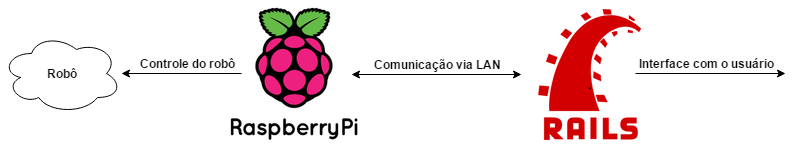
\includegraphics[scale=0.50, angle = 360]{figuras/arquitetura_1}
\caption[]{Arquitetura do sistema (fonte: Autor)}
\end{figure}
\FloatBarrier

O fluxo de execução do sistema pode ser resumido a seguir:

\begin{enumerate}
    \item O bibliotecário interage com a interface \textit{web} para realizar algum tipo de atividade administrativa (adicionar um livro ao acervo, devolução de livros, empréstimo, etc…). Cada uma dessas atividades administrativas exige um gerenciamento interno do sistema \textit{web} para identificar o estado das estantes (quais posições estão sendo utilizadas, por exemplo) e dos livros (quais livros estão disponíveis e onde estão armazenados). Para isso, a aplicação \textit{web} contará com uma base de dados que será responsável por armazenar estas informações. Por fim, o portal da biblioteca enviará requisições ao software sendo executado na \textit{Raspberry Pi} informando algum tipo de ação a ser executada.

    \item O servidor sendo executado na \textit{Raspberry Pi} aceitará requisições do portal da biblioteca e mapeará uma requisição a uma série de comandos que especificam ao robô as ações que devem ser tomadas para cumprir a função solicitada.

    \item As funções do robô são acionadas a partir do \textit{software} embarcado na \textit{Raspberry Pi} e após seu término, o servidor envia uma resposta ao portal da biblioteca notificando a conclusão da solicitação enviada.

    \item O portal informa ao usuário que a função solicitada foi executada.
\end{enumerate}

\section{Metas e Restrições da Arquitetura}
Existem algumas metas e restrições arquiteturais consideradas relevantes pela equipe de desenvolvimento, são elas:

\begin{enumerate}
    \item A aplicação \textit{web} será executada em uma rede local, pois não faz sentido a atribuição de um IP público se ela só será acessada pelos funcionários da biblioteca e se comunicará com o servidor da \textit{Raspberry Pi} que também pertence à rede local.

    \item O portal da biblioteca deve apresentar um sistema de identificação e autenticação que garanta que apenas funcionários autorizados possam acessá-lo com sucesso.

    \item O servidor da \textit{Raspberry Pi} deve aceitar requisições exclusivamente do portal da biblioteca.

    \item A implantação do sistema em uma organização deve ser automatizada, para evitar a configuração manual de IPs para viabilizar a comunicação entre os subsistemas de \textit{software}.
\end{enumerate}

\section{Visão Lógica}
Esta seção se concentra em descrever detalhes arquiteturais internos de cada subsistema:

\begin{enumerate}
    \item\textbf{Sistema \textit{web}:} O sistema \textit{web} será implementado utilizando o estilo arquitetural MVC (\textit{Model}, \textit{View}, \textit{Controller}). Este padrão arquitetural determina a subdivisão do \textit{software} em camadas com responsabilidades específicas:

    \subitem\textbf{Model:} responsável por representar as entidades envolvidas no projeto e implementar a interface entre o sistema e a base de dados.

    \subitem\textbf{View:} responsável por conter o código relacionada à camada visual da aplicação.

    \subitem\textbf{Controller:} responsável por coordenar o fluxo de execução do sistema e atuar como a interface entre as camadas descritas anteriormente.
    
    A aplicação \textit{web} também será responsável por administrar o uso das estantes. Para isso, o projeto implementa um recurso de discretização das estantes. A discretização é possibilitada pela construção de cases de tamanho único que irão envolver os livros, dessa forma, o espaço ocupado por cada livro é determinístico e o \textit{software} é capaz de interpretar a estante como uma matriz binária, onde cada posição da estante pode ser representada por um par ordenado. Este par ordenado será armazenado para identificar a posição exata de um determinado livro.


    \item\textbf{Sistema Embarcado:} O sistema embarcado será dividido em dois módulos principais:

    \subitem\textbf{Servidor:} responsável por aceitar requisições do sistema \textit{web} e processá-las para identificar quais comandos devem ser enviados para o robô, além de enviar mensagens de resposta informando ao portal o estado da execução da tarefa solicitada.

    \subitem\textbf{Controlador: } responsável por enviar comandos para o robô para acionar suas funções. Cada função do robô está associada a um dispositivo externo, por exemplo, um motor de passo. Estes dispositivos são representados internamente por um arquivo de dispositivo. A comunicação entre o \textit{software} e os dispositivos periféricos será realizada através destes arquivos e da interface de programação unificada fornecida por sistemas Unix-like para manipulação de arquivos.
    
\end{enumerate}



